

\section{Introduction} 
% Section outline:
% Overall summary of project - ~1 sentence per major goal
% ~1 Paragraph for each major goal
% Paragraph at end describing what is in this document

%Designed by Kevin Harrington in Bowler Studio
\subsection{Problem Statement}
\noindent Currently, it is difficult for users to fully understand the motion of robotic arms and the kinematics that control them. This understanding is a crucial step in working with robotic arms safely and efficiently, but is often lacking due to the inability of diagrams and descriptions to fully convey what makes one arm operate differently than another. With the use of robotic arms becoming more common and the many different kinds of arms available, it is important to have a prototyping platform that can emulate many different kinds of arms so that the user can gain a better grasp of what components make up a robotic arm why one arm is better suited for a particular use case than another.

\subsection{Goal Statement}
The goal of this project is to create a proof of concept of an arm that can be reconfigured by end users such that they can create many different types of functionality from one set of principal components. To accomplish this, we need to break the arm down into small modularized joints that can be rearranged to show how the combination of different kinds of joints can lead to a specific end result. We also need to create an adaptable electrical system that is able to modularly control each different joint by having the capability to handle multiple types of sensors and actuators. By doing so, we hope to take the first step into creating a standardized kit of parts and the software accompanying it to prototype almost any type of arm that is currently used. 

\subsection{Objectives}
\noindent In order to measure our progress, we define a set of objectives that we need to accomplish in order to meet our goals outlined above. To create a proof of concept of a modular robotic arm prototyping platform, we set the following objectives: 
%\newline \noindent \textbf{Objectives}
\begin{itemize}
\item Define commonly used robotic arms and their uses.
\item Understand the variety of different joints and what sensors and actuators are used to control them.
\item Understand how the combinations of different joints affects the kinematics of the arm.
\item Classify several different standardized joints and what sensors/actuators make them work.
\item Create a control bus made up of connected joints with a node at each joint capable of controlling any single joint.
\item Create a joint that can be added and removed from an existing arm in order to modify the arm's functionality.
\item Create an arm control board which functions as an interface between a computer and our arm's control bus allowing for users to interact with the arm through a software interface.
\item Create a software application which displays information about the arm in real time and allows users to easily set up their arm and send it commands.
\end{itemize} 

\subsection{Constraints}
\noindent In order to complete this project in the alloted time, we had to place limits on our goals for the project. One such constraint was taking into account the time it would take to prototype, design and assemble a fully modular arm from scratch. Changes in the project's organizational structure led us to revise our goals (the original ones of which are reflected in Appendix \ref{app:Early-Project-Iteration}) To handle this, we decided that we could show off a smaller-scale example of modularity by modifying an existing arm by adding a joint that can be easily removed. By fully creating our own link that can be attached to the arm to increase utility, we proved that the idea of a modular joint is feasible and therefore those joints can be combined to create a modular arm. We also had to impose another constraint to ensure proper functionality of the arm which is that the arm can have at maximum six joints controlled at once. This constraint was decided based upon examples of other robotic arms as well as a way to make sure that the arm is structurally sound and within weight tolerances.

\subsection{Summary}
\noindent Once we outlined our goals and constraints for the project, we had a clear idea of where to start researching. Knowing what we have to accomplish as well as knowing the obstacles standing in our way, we were able to approach the project piece by piece, working towards our goals as well as keeping a solid perspective about the entire scope of the project. When we ran into design decisions that were not foreseeable before we got working, we referred back to our original goals and based our decisions off of these initial measures of project progress. Moving forward after defining the problem fully and how we wanted to accomplish it, we proceeded to conduct research on current robotic arm technology that we used as a reference for our arm.  

%The goal of this project was to create an adaptable control system whose purpose is to drive a variety of robotic arms. To prove the usefulness of our system, we retrofitted an existing robot arm from the RBE 3001 course with our control system. In addition to this, we modified the existing arm to include an interchangeable joint on the end of our arm, controlled by our system. To interface with our system, we created a GUI for easy configuration and basic control of the arm. The base communicates with a computer running control code through the software application. \\
%\newline
%
%\begin{figure}[H]
%\centering
%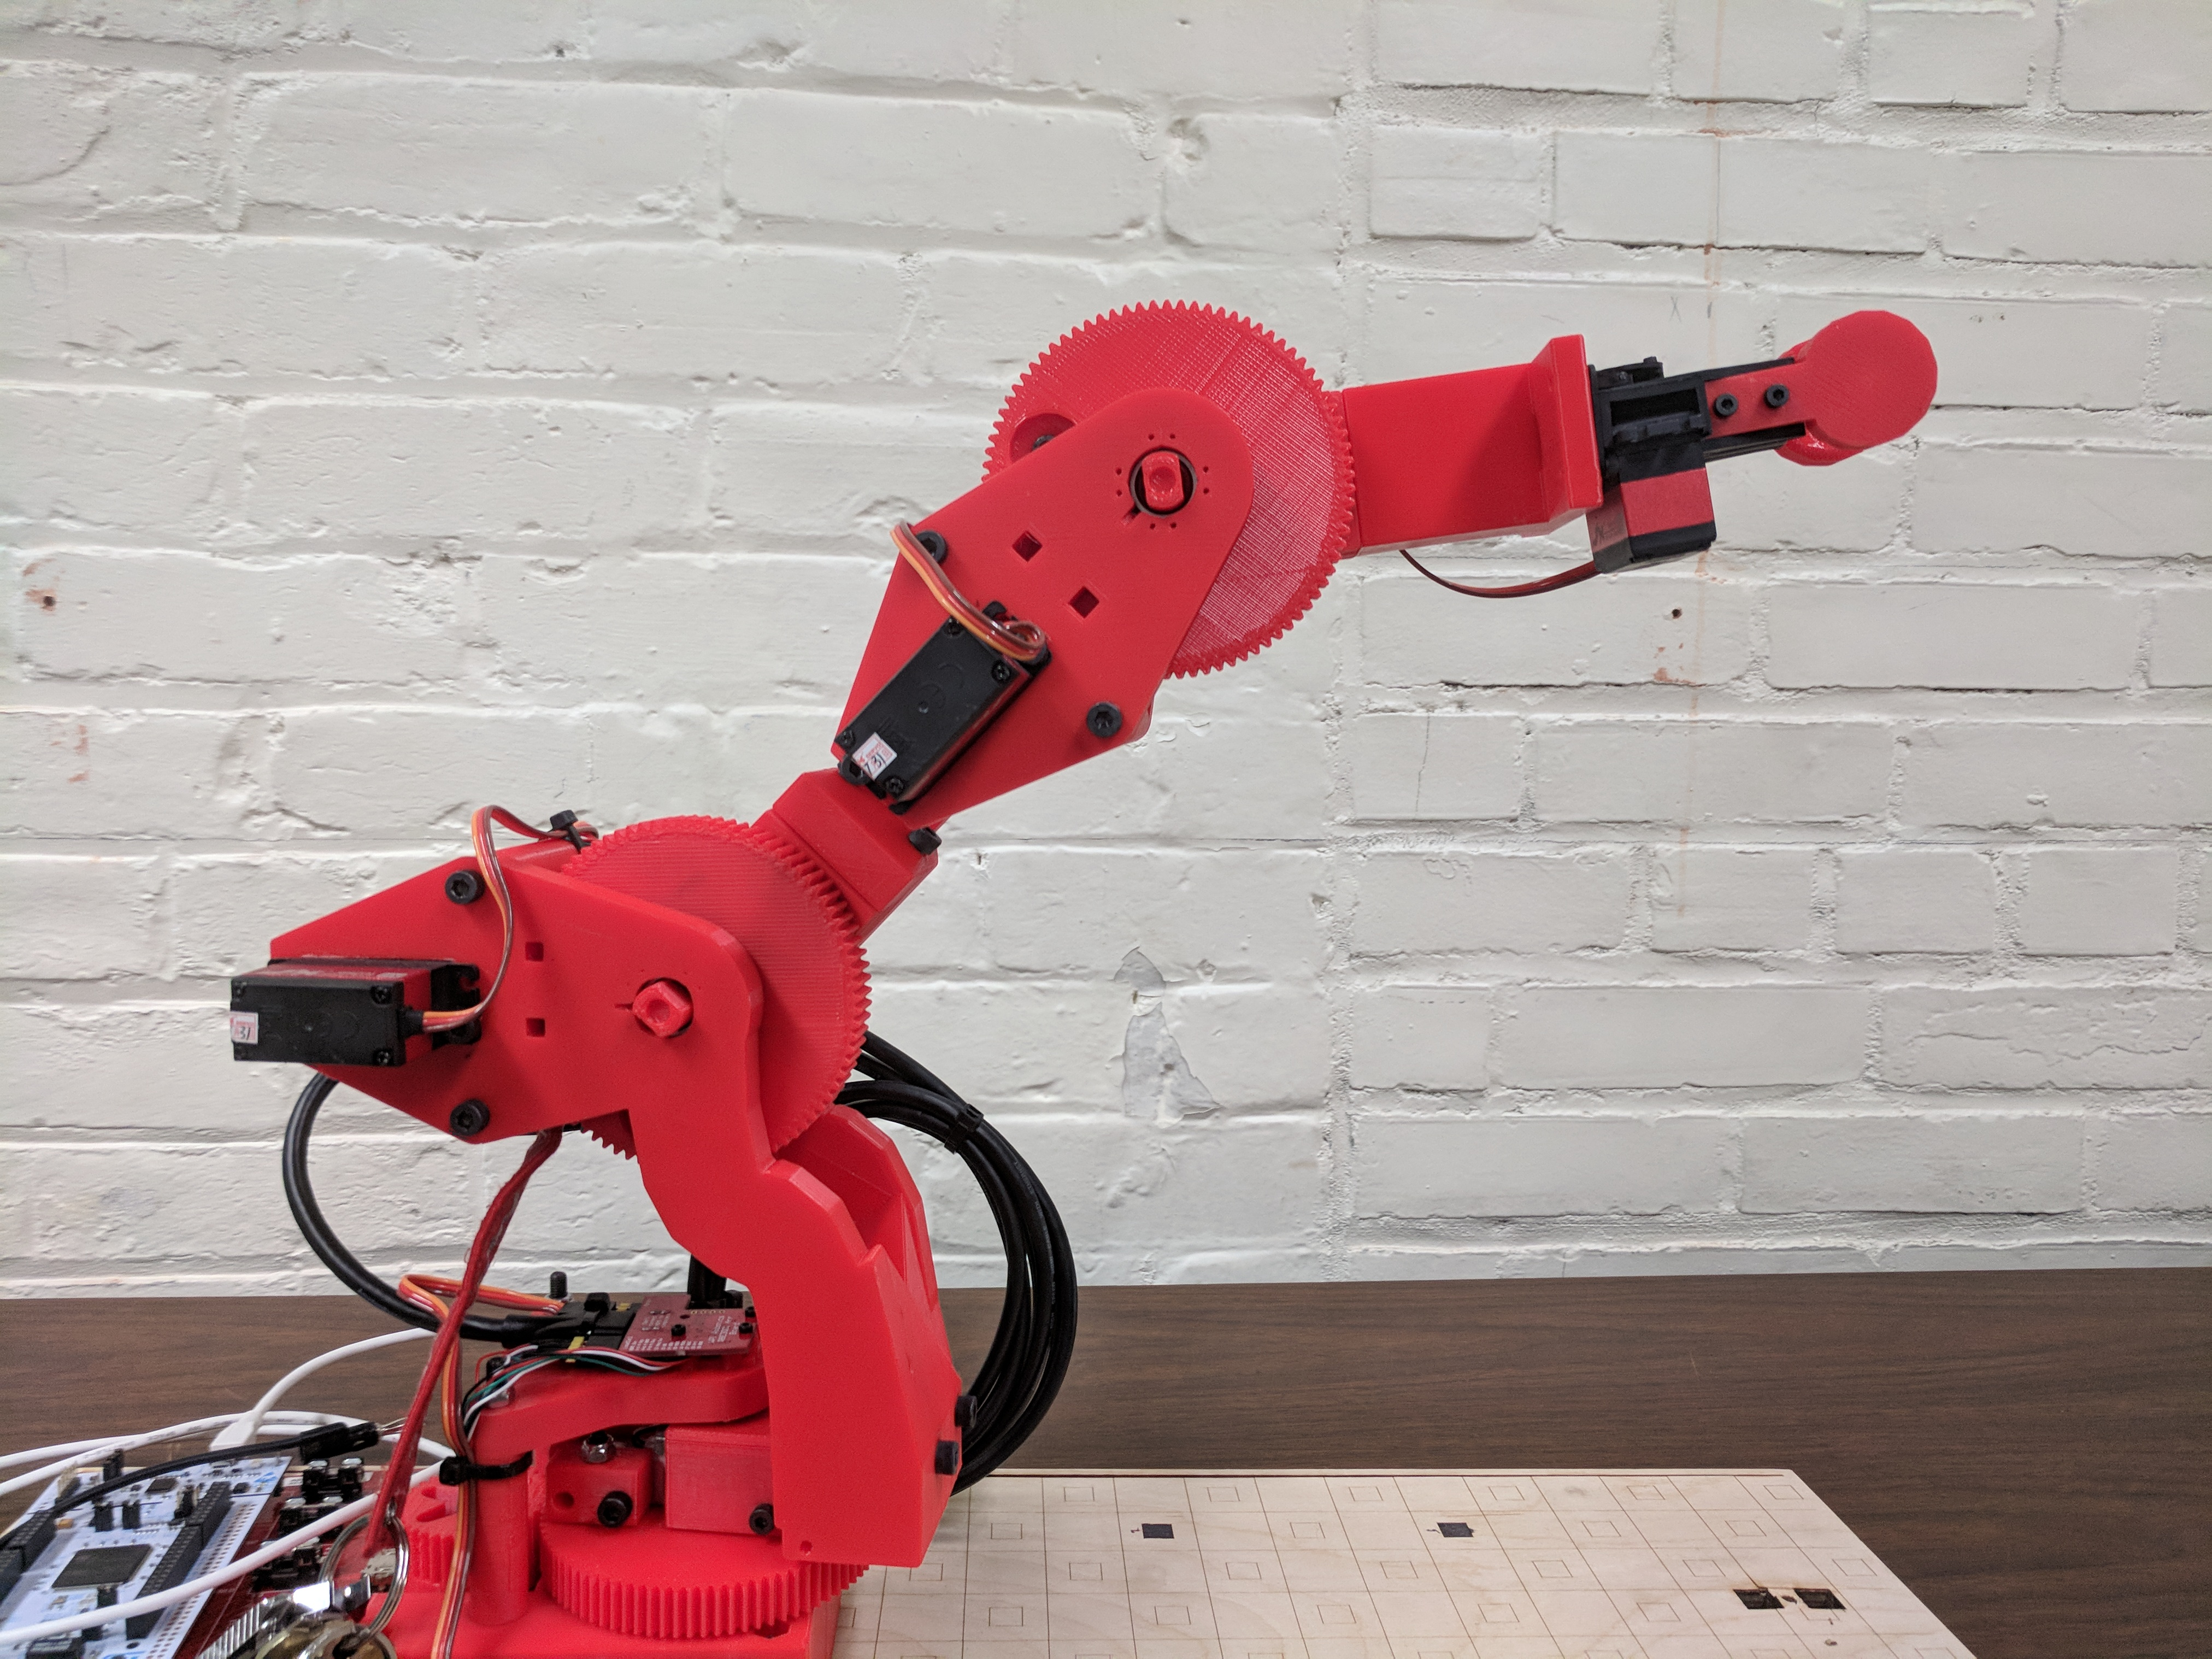
\includegraphics[width=\textwidth]{Initial_3001_Arm}
%\caption{Unmodified RBE 3001 Arm}
%\label{fig:3001_Arm}
%\end{figure}
%
%
%
%\noindent The existing RBE 3001 arm already has its own central control system. We removed this and replaced it with our own distributed one. To accomplish this, we designed a joint control board that communicates with a base controller.  We also designed and implemented a new joint on the arm. This new joint is interchangeable to prove that our software and control system will work with more than one configuration. The joint implements our control board. \\
%\newline
%We created a software application to interface with a constructed arm. The user inputs how they have configured their arm into this application and are then able to do some simple control. Another feature of this application is the ability to record a series of poses for the arm to perform. In addition to this software, we also created some programming libraries to allow users to control the arm with their own programs. \\
%\newline
%In this document, we will outline some existing robot arms and highlight the differences between these arms and our arm kit. We then discuss what work there is to be done on this project. After discussing the work to be done, we state how this work will satisfy the capstone design requirements for each of the three disciplines represented by our group members. Then, we state the constraints we expect going forward with this project. Next, the acceptance criteria for any deliverables at the end of this project will be outlined. Finally, we will state an estimated time line for this project. Additionally, due to changes in project organization we have significantly changed the scope and goals of the project. See Appendix \ref{app:Early-Project-Iteration} for more information about this earlier iteration of our project.